\documentclass[10pt]{beamer}

% \usetheme[progressbar=frametitle]{metropolis}
\usepackage{appendixnumberbeamer}
\usecolortheme{orchid}

\usepackage{booktabs}
\usepackage[scale=2]{ccicons}

\usepackage{pgfplots}
\usepgfplotslibrary{dateplot}

\usepackage{xspace}
% \newcommand{\themename}{\textbf{\textsc{metropolis}}\xspace}

% For caption without labels
\usepackage{caption}
\captionsetup{font=tiny}
\setbeamertemplate{caption}{\raggedright\insertcaption\par}

% \usefonttheme{professionalfonts}
% \usefonttheme{serif}

\title{Bi-Fidelity Data-assisted Neural Networks in Nonintrusive Reduced Order Modeling}
% \subtitle{}
\date{April 22, 2019}
\author{Chuan Lu}
% \institute{}
\titlegraphic{\hfill
\includegraphics[height=1.5cm]{DomeWordPrimaryBLACK.eps}}

\begin{document}

\maketitle

% \begin{frame}{Table of contents}
%   \setbeamertemplate{section in toc}[sections numbered]
%   \tableofcontents[hideallsubsections]
% \end{frame}

% \section{Introduction}

% \section{High-fidelity simulations}
\begin{frame}{High-fidelity simulations}

\begin{itemize}
\item Formalized as parameterized PDEs
\item Indispensible in science and engineering
\item Require great computational cost, especially for many-query and real-time situations
\end{itemize}

\begin{figure}
\centering
  \begin{minipage}[t]{0.32\textwidth}
    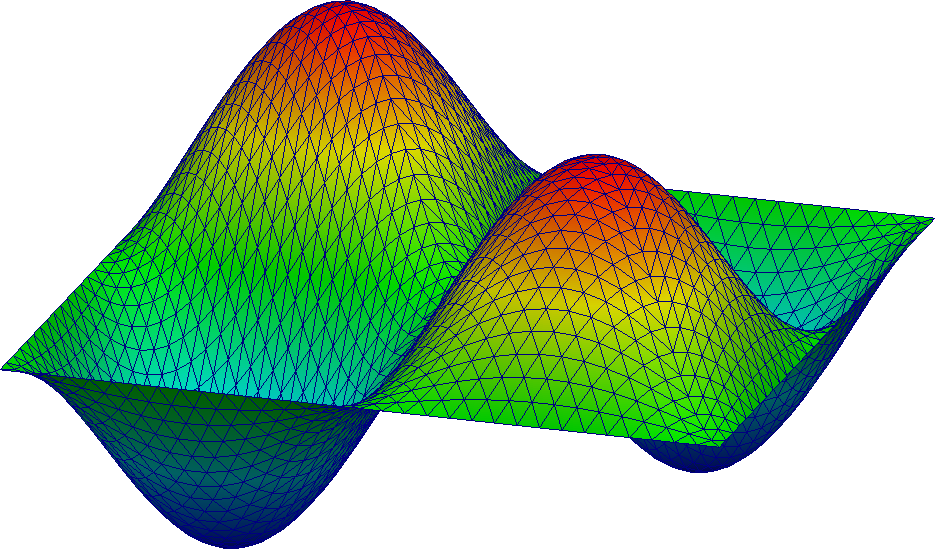
\includegraphics[width=\textwidth]{figures/Lapl2D_4.png}
    \footnotemark[1]
    \caption{2D Laplace equation}
  \end{minipage}
  \begin{minipage}[t]{0.32\textwidth}
    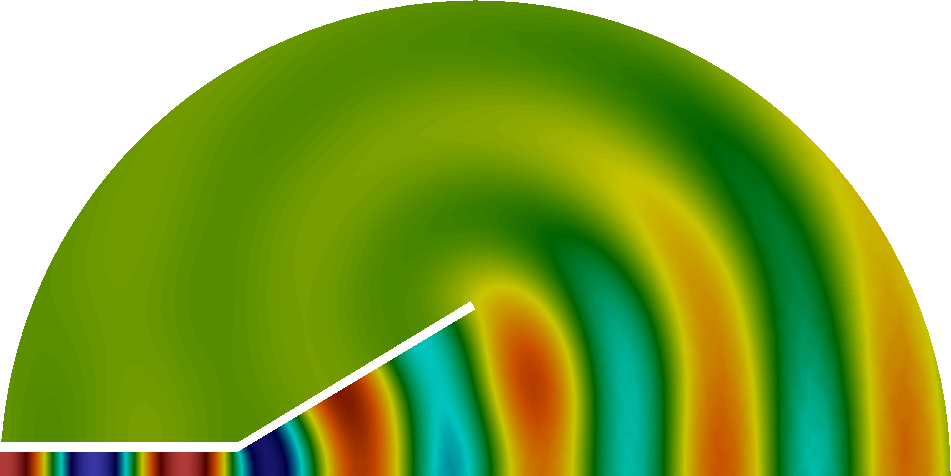
\includegraphics[width=\textwidth]{figures/AcousticHorn.png}
    \footnotemark[1]
    \caption{2D Helmholtz equation}
  \end{minipage}
  \begin{minipage}[t]{0.32\textwidth}
    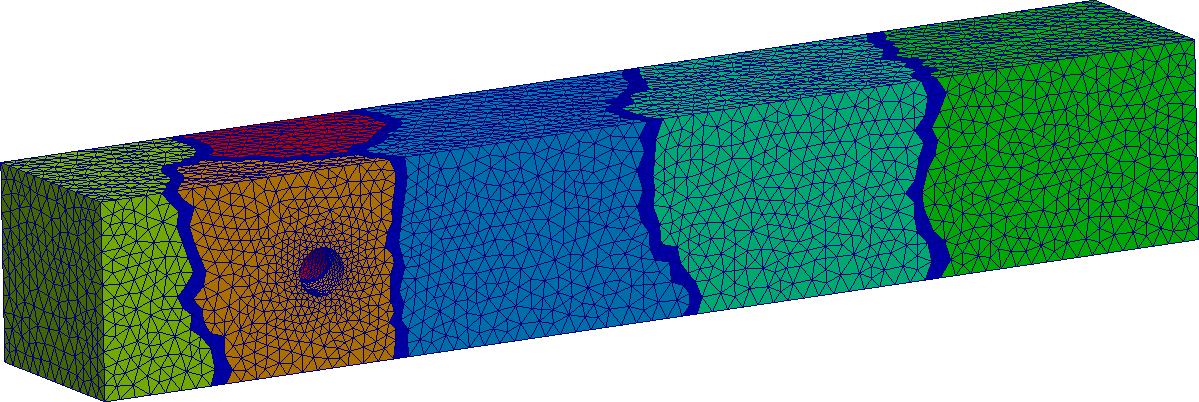
\includegraphics[width=\textwidth]{figures/Dfg3D_DD_2.png}
    \footnotemark[1]
    \caption{3D Navier-Stokes equation}
  \end{minipage}
\end{figure}
\footnotetext[1]{\tiny A. Quarteroni, A. Manzoni and F. Negri.
Reduced Basis Methods for Partial Differential Equations. An Introduction.
Unitext, vol. 92. Springer, 2016. https://redbkit.github.io/redbKIT/}
\end{frame}


\begin{frame}{Problem setup}
Parameterized PDE:
$$
\left\{
\begin{aligned}
&\mathcal{L}u(x, z) = f, \quad \text{in}\ D, \\ 
&u(x, z) = g, \quad \text{on}\ \partial D.
\end{aligned}
\right.
$$
Many-query problem: solve the PDE for $z \in Z_{query} \subset I_{z} $.

\end{frame}

\begin{frame}{Proper Orthogonal Decomposition (POD)}
\begin{itemize}
  \item Seek for a set of parameter-independent function basis for the full-order solution space
  \item Minimize the $L_2 $ error
\end{itemize}

\begin{block}{POD}
\begin{enumerate}
\item Generate a full-order snapshot matrix $S = [u(x, z_1), \hdots, u(x, z_P)].$
\item At dimension $k$, pick the first $k$ left singular vectors of $S$ to form the basis $V$ of the reduced space.
\item Compute the reduced approximation by projection onto the reduced space: $c_{rb}(z) = V^\top u(x, z), \ u_{rb}(x, z) = Vc_{rb} $.
\end{enumerate}
\end{block}
For nonintrusive methods, at the online stage, the coefficients $c_{rb}(z^*) $ are recovered without the projection of the full-order solution.


\end{frame}

\begin{frame}{POD-NN}
Use neural networks to learn the mapping $z \to c_{rb}(z)$\cite{hesthaven2018non}.
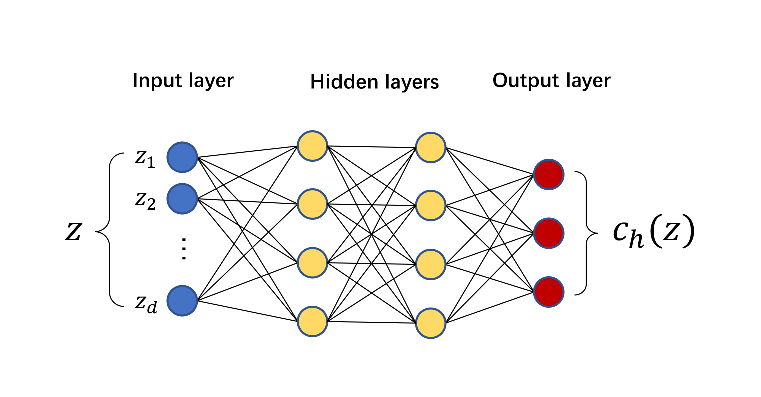
\includegraphics[scale=0.6]{figures/PODNN.pdf}

\begin{itemize}
\item For nonlinear problems, POD-NN has a good performance because of the nonlinear nature of neural networks.
\end{itemize}

\end{frame}

\begin{frame}{Low-fidelity models}
\begin{itemize}
\item Common in scientific and engineering applications
\item Inaccurate, but can mimic important behaviours of the problem
\item Much lower computational cost
\end{itemize}

\end{frame}

\begin{frame}{BiFi-NN}
\begin{itemize}
\item We incorporate additional features extracted from the low-fidelity model to the input of POD-NN\cite{lu2019bifidelity}.
\item One possible choice is to use the low-fidelity POD coefficients. 
\end{itemize}

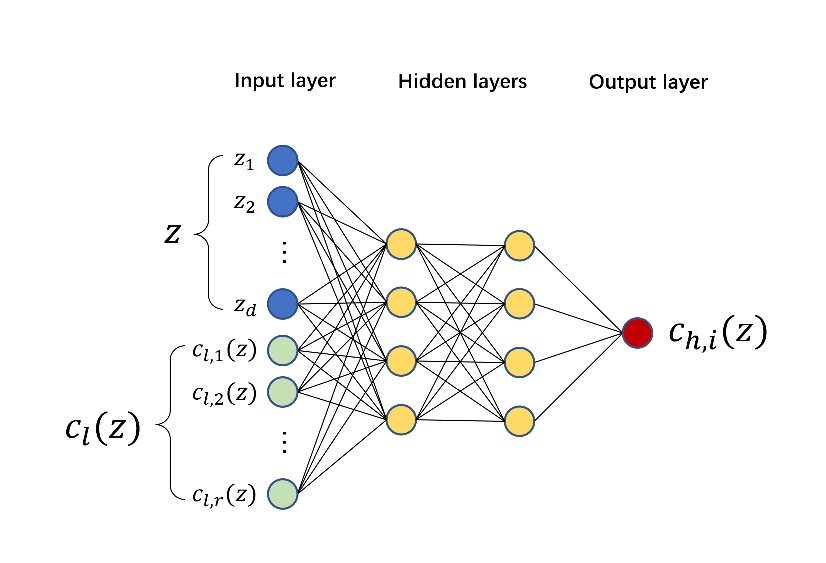
\includegraphics[scale=0.6]{figures/BFNN.pdf}

\end{frame}

\begin{frame}{BiFi-NN (cont.)}
Two problems with BiFi-NN:
\begin{itemize}
\item In the offline stage, it needs a large collection of high-fidelity snapshots to generate the POD basis.
\item In the online stage, it requires one additional low-fidelity simulation to extract the additional input feature.

\end{itemize}
\pause

To tackle these challenges, we apply the following methods:
\begin{itemize}
\item Apply a point selection method to the low-fidelity snapshots to select a subset of parameters for generating the high-fidelity POD basis.
\item Use a two-step prediction scheme, i.e., use another network to approximate the low-fidelity POD coefficients instead of the real ones.
% \item Use Cholesky selection (or rank-revealing QR) on the low-fidelity snapshot collection to select a subset of parameters, and simulate the high-fidelity models on this subset. This high-fidelity snapshot collection is then used to generate the POD basis for the high-fidelity model.
% \item Generate an additional set of low-fidelity snapshots,
\end{itemize}
\end{frame}

\begin{frame}{Point selection}
\begin{block}{}
\begin{enumerate}
\item Simulate the low-fidelity model on a set of parameters $Z\subset I_z $.
\item Use point selection methods to select a subset $\tilde{Z}\subset Z $.
\item Simulate the high-fidelity model on $\tilde{Z}$ and compute the POD basis.
\end{enumerate}
\end{block}

In this project, we use Cholesky selection method\cite{zhu2014computational}. Alternative methods include rank-revealing QR (RRQR).

\end{frame}

\begin{frame}{Two-step prediction}
\centering
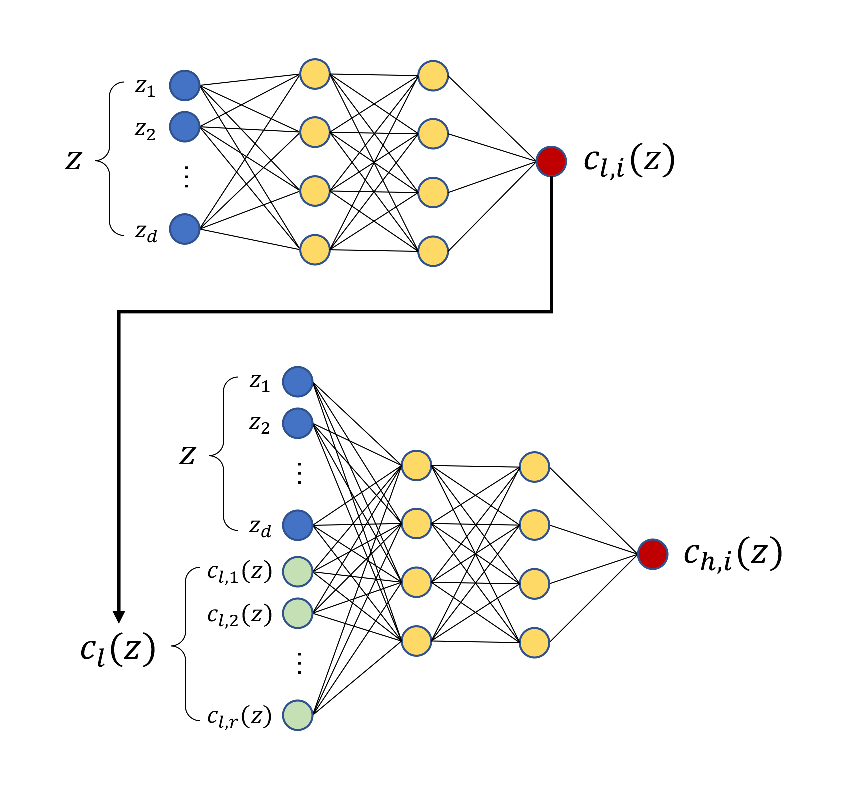
\includegraphics[scale=0.5]{figures/Two-step.pdf}

Online complexity: $O(S+F) \to O(2F)$.
\end{frame}

% \begin{frame}{Algorithm}
% \begin{enumerate}
% \item Sample a set of parameters $Z\subset I_z $, and compute the low-fidelity models $u_l(z)$ for each $z$


% \end{enumerate}
% \end{frame}
\begin{frame}{2D Vorticity Equation}
$$
\left\{
\begin{aligned}
&\partial_t w = \mu\Delta w-(u\cdot\nabla)w, \ (x, y, \mu)\in [0, 2\pi]\times [0, 2\pi]\times [2\times 10^{-3}, 5\times 10^{-3}], \\
&w|_{t=0} = \hat{w}+\epsilon(x, y),
\end{aligned}
\right.
$$
where $w = \nabla\times u$, 
$$
\begin{aligned}
    \hat{w}((x, y),0)&= \exp\left(-\frac{(x-\pi+\pi/5)^2+(y-\pi+\pi/5)^2}{0.3}\right) \\
    &\ -\exp\left(-\frac{(x-\pi-\pi/5)^2+(y-\pi+\pi/5)^2}{0.2}\right) \\
    &\ +\exp\left(-\frac{(x-\pi-\pi/5)^2+(y-\pi-\pi/5)^2}{0.4}\right), \\
\end{aligned}
$$
and $\epsilon$ is a random noise uniformly distributed in [-1, 1]. We use Fourier spectral method to solve this problem until final time $T = 50$ with timestep $\Delta t = 0.1$.

\end{frame}

\begin{frame}{2D Vorticity Equation (cont.)}
\begin{itemize}
\item High-fidelity model: solved on a uniform grid of size $128\times 128$ with average running time 7.73s.
\item Low-fidelity model: solved on a uniform grid of size $16\times 16$, with average running time 0.39s.
\item For POD-NN and BiFi-NN, we use 300 independent snapshots to generate the high-fidelity POD basis; for BiFi-NN with Cholesky selection, only 26 values of the parameter are chosen from the low-fidelity snapshots. Thus, we reduced the number of high-fidelity snapshots for generating POD basis by 274.
\end{itemize}  
\end{frame}

\begin{frame}{2D Vorticity Equation (cont.)}
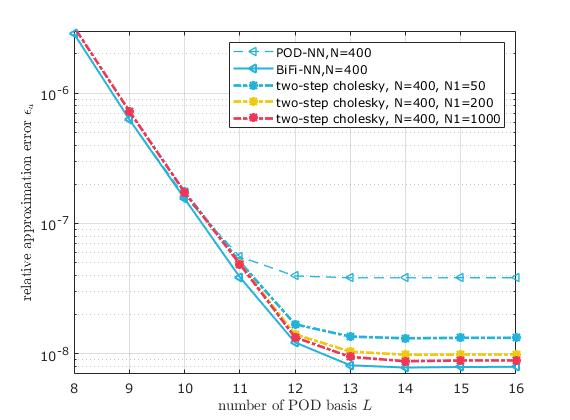
\includegraphics[scale=0.5]{figures/two_step.jpg}

\end{frame}


\begin{frame}[allowframebreaks]{References}

  \bibliography{slide}
  \bibliographystyle{abbrv}

\end{frame}

\end{document}
